\section{Model3D  Class Reference}
\label{class_Model3D}\index{Model3D@{Model3D}}
A base class for all models in 3D worlds. 


{\tt \#include $<$model3d.h$>$}

Inheritance diagram for Model3D::\begin{figure}[H]
\begin{center}
\leavevmode
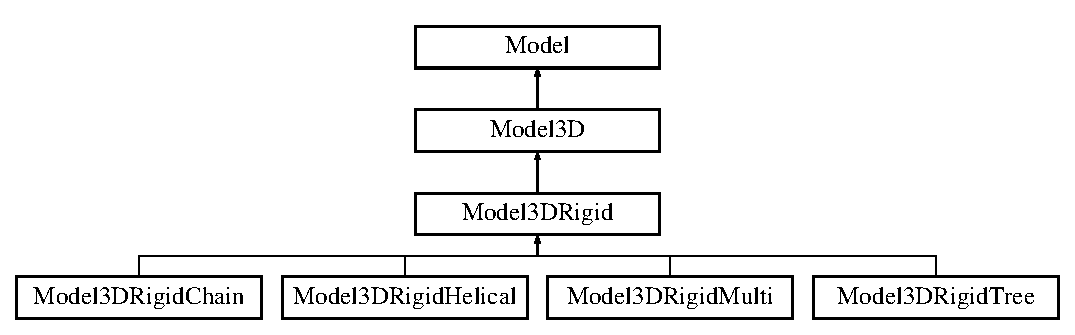
\includegraphics[height=4cm]{class_Model3D}
\end{center}
\end{figure}
\subsection*{Public Methods}
\begin{CompactItemize}
\item 
{\bf Model3D} (string path)
\item 
virtual {\bf $\sim$Model3D} ()
\end{CompactItemize}


\subsection{Detailed Description}
A base class for all models in 3D worlds.



\subsection{Constructor \& Destructor Documentation}
\index{Model3D@{Model3D}!Model3D@{Model3D}}
\index{Model3D@{Model3D}!Model3D@{Model3D}}
\subsubsection{\setlength{\rightskip}{0pt plus 5cm}Model3D::Model3D (string {\em path})}\label{class_Model3D_a0}


\index{Model3D@{Model3D}!~Model3D@{$\sim$Model3D}}
\index{~Model3D@{$\sim$Model3D}!Model3D@{Model3D}}
\subsubsection{\setlength{\rightskip}{0pt plus 5cm}Model3D::$\sim$Model3D ()\hspace{0.3cm}{\tt  [inline, virtual]}}\label{class_Model3D_a1}




The documentation for this class was generated from the following file:\begin{CompactItemize}
\item 
{\bf model3d.h}\end{CompactItemize}
